介绍SRAM和DRAM之前,首先了解半导体存储芯片的基本结构及其译码驱动方式。

\textbf{{1.半导体存储芯片的基本结构}}\\

半导体存储芯片主要由存储矩阵、译码驱动电路和读/写电路组成,如下图所示。

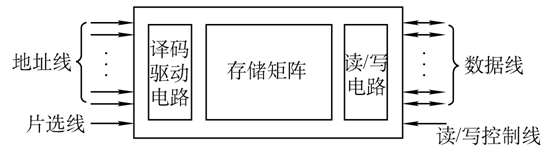
\includegraphics[width=3.69792in,height=1.03125in]{png-jpeg-pics/ED2922D02AD866CAA8E42D2CDF94FAC7.png}

从上图中可以看出,\textbf{地址线是单向的,数据线是双向的,}剩下的属于控制线,控制线有读/写控制线和片选线两种。读/写控制线用来进行读/写操作,片选线用来选择存储芯片。由于一般半导体都是由很多的芯片组成的,因此需要用片选信号来选择要读或写哪一个芯片。

\textbf{{2.半导体存储芯片的译码驱动方式}}

\textbf{半导体存储芯片的译码驱动方式分为两种:线选法和重合法。}

\textbf{(1)线选法(单译码)}

首先假设该矩阵有N行,然后就可以通过公式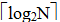
\includegraphics[width=0.41667in,height=0.15625in]{png-jpeg-pics/FB018EBBCBADD70A7F1EBBA64FA6D211.png}算出地址线所需要的根数。以下图为例,矩阵有16行,需要4根地址线A0、A1、A2、A3,值0000,0001,0010,,1111共16个数,分别代表了该矩阵的16行。由于图3-5中A0、A1、A2、A3的值都为0,因此选中了第0行。选中之后再由读/写控制电路进行读写操作即可。另外,由于矩阵每行有8位,因此需要8根数据线。

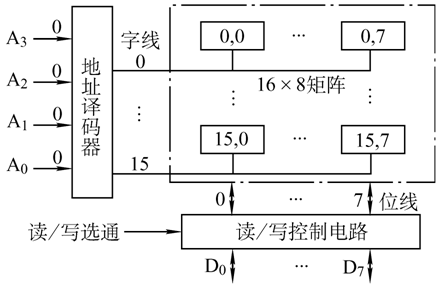
\includegraphics[width=3.69792in,height=2.43750in]{png-jpeg-pics/0A06B53A95A27FD6C136C69CA2915CB8.png}

\textbf{(2)重合法(双译码)}

\textbf{线选法}是选中矩阵的一行(在计算机中称为选中一个字),而\textbf{重合法}比线选法更细,它可以选中矩阵的某一个元素(在计算机中称为选中一位)。如下图所示,存储矩阵可以看成是3232的矩阵。由线性代数可知,要想在矩阵中定位一个元素,需要行列的坐标,故此时不但需要行地址线,而且还需要列地址线。32行里选中一行需要5根地址线,32列里选中一列也需要5根地址线,一共需要10根地址线。图3-6中10根地址线全为0,就选中了矩阵的(0,0)元素。

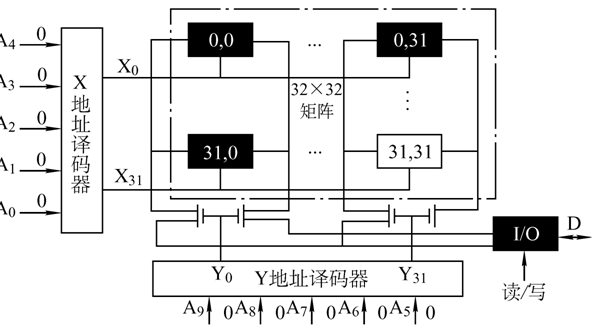
\includegraphics[width=3.69792in,height=2.06250in]{png-jpeg-pics/447C0262C0FFF357F20348C35B08E9FB.png}
